%!TEX TS-program = xelatex

% Шаблон документа LaTeX создан в 2018 году
% Алексеем Подчезерцевым
% В качестве исходных использованы шаблоны
% 	Данилом Фёдоровых (danil@fedorovykh.ru) 
%		https://www.writelatex.com/coursera/latex/5.2.2
%	LaTeX-шаблон для русской кандидатской диссертации и её автореферата.
%		https://github.com/AndreyAkinshin/Russian-Phd-LaTeX-Dissertation-Template

\documentclass[a4paper,14pt]{article}

%%% Работа с русским языком
\usepackage[english,russian]{babel}   %% загружает пакет многоязыковой вёрстки
\usepackage{fontspec}      %% подготавливает загрузку шрифтов Open Type, True Type и др.
\defaultfontfeatures{Ligatures={TeX},Renderer=Basic}  %% свойства шрифтов по умолчанию
\setmainfont[Ligatures={TeX,Historic}]{Times New Roman} %% задаёт основной шрифт документа
\setsansfont{Comic Sans MS}                    %% задаёт шрифт без засечек
\setmonofont{Courier New}
\usepackage{indentfirst}
\frenchspacing

\renewcommand{\epsilon}{\ensuremath{\varepsilon}}
\renewcommand{\phi}{\ensuremath{\varphi}}
\renewcommand{\kappa}{\ensuremath{\varkappa}}
\renewcommand{\le}{\ensuremath{\leqslant}}
\renewcommand{\leq}{\ensuremath{\leqslant}}
\renewcommand{\ge}{\ensuremath{\geqslant}}
\renewcommand{\geq}{\ensuremath{\geqslant}}
\renewcommand{\emptyset}{\varnothing}

%%% Дополнительная работа с математикой
\usepackage{amsmath,amsfonts,amssymb,amsthm,mathtools} % AMS
\usepackage{icomma} % "Умная" запятая: $0,2$ --- число, $0, 2$ --- перечисление

%% Номера формул
%\mathtoolsset{showonlyrefs=true} % Показывать номера только у тех формул, на которые есть \eqref{} в тексте.
%\usepackage{leqno} % Нумерация формул слева	

%% Перенос знаков в формулах (по Львовскому)
\newcommand*{\hm}[1]{#1\nobreak\discretionary{}
	{\hbox{$\mathsurround=0pt #1$}}{}}

%%% Работа с картинками
\usepackage{graphicx}  % Для вставки рисунков
\graphicspath{{images/}}  % папки с картинками
\setlength\fboxsep{3pt} % Отступ рамки \fbox{} от рисунка
\setlength\fboxrule{1pt} % Толщина линий рамки \fbox{}
\usepackage{wrapfig} % Обтекание рисунков текстом

%%% Работа с таблицами
\usepackage{array,tabularx,tabulary,booktabs} % Дополнительная работа с таблицами
\usepackage{longtable}  % Длинные таблицы
\usepackage{multirow} % Слияние строк в таблице
\usepackage{float}% http://ctan.org/pkg/float

%%% Программирование
\usepackage{etoolbox} % логические операторы


%%% Страница
\usepackage{extsizes} % Возможность сделать 14-й шрифт
\usepackage{geometry} % Простой способ задавать поля
\geometry{top=20mm}
\geometry{bottom=20mm}
\geometry{left=20mm}
\geometry{right=10mm}
%
%\usepackage{fancyhdr} % Колонтитулы
% 	\pagestyle{fancy}
%\renewcommand{\headrulewidth}{0pt}  % Толщина линейки, отчеркивающей верхний колонтитул
% 	\lfoot{Нижний левый}
% 	\rfoot{Нижний правый}
% 	\rhead{Верхний правый}
% 	\chead{Верхний в центре}
% 	\lhead{Верхний левый}
%	\cfoot{Нижний в центре} % По умолчанию здесь номер страницы

\usepackage{setspace} % Интерлиньяж
\onehalfspacing % Интерлиньяж 1.5
%\doublespacing % Интерлиньяж 2
%\singlespacing % Интерлиньяж 1

\usepackage{lastpage} % Узнать, сколько всего страниц в документе.

\usepackage{soul} % Модификаторы начертания

\usepackage{hyperref}
\usepackage[usenames,dvipsnames,svgnames,table,rgb]{xcolor}
\hypersetup{				% Гиперссылки
	unicode=true,           % русские буквы в раздела PDF
	pdftitle={Автоматизация проектных работ},   % Заголовок
	pdfauthor={Солодянкин А.А.},      % Автор
	pdfsubject={Автоматизация проектных работ},      % Тема
	pdfcreator={Солодянкин А.А.}, % Создатель
	pdfproducer={Солодянкин А.А.}, % Производитель
	pdfkeywords={Автоматизация проектных работ}, % Ключевые слова
	colorlinks=true,       	% false: ссылки в рамках; true: цветные ссылки
	linkcolor=black,          % внутренние ссылки
	citecolor=black,        % на библиографию
	filecolor=magenta,      % на файлы
	urlcolor=black           % на URL
}
\makeatletter 
\def\@biblabel#1{#1. } 
\makeatother
\usepackage{cite} % Работа с библиографией
%\usepackage[superscript]{cite} % Ссылки в верхних индексах
%\usepackage[nocompress]{cite} % 
\usepackage{csquotes} % Еще инструменты для ссылок

\usepackage{multicol} % Несколько колонок

\usepackage{tikz} % Работа с графикой
\usepackage{pgfplots}
\usepackage{pgfplotstable}

% ГОСТ заголовки
\usepackage[font=small]{caption}
%\captionsetup[table]{justification=centering, labelsep = newline} % Таблицы по правобу краю
%\captionsetup[figure]{justification=centering} % Картинки по центру


\newcommand{\tablecaption}[1]{\addtocounter{table}{1}\small \begin{flushright}\tablename \ \thetable\end{flushright}%	
\begin{center}#1\end{center}}

\newcommand{\imref}[1]{рис.~\ref{#1}}

\usepackage{multirow}
\usepackage{spreadtab}
\newcolumntype{K}[1]{@{}>{\centering\arraybackslash}p{#1cm}@{}}


\usepackage{xparse}
\usepackage{fancyvrb}

\RecustomVerbatimCommand{\VerbatimInput}{VerbatimInput}
{
	fontsize=\footnotesize    
}

\newcolumntype{?}[1]{!{\vrule width #1}}

\usepackage{tocloft}
\renewcommand{\cftsecleader}{\cftdotfill{\cftdotsep}}
\begin{document} % конец преамбулы, начало документа
\begin{titlepage}
	\begin{center}
		ПРАВИТЕЛЬСТВО РОССИЙСКОЙ ФЕДЕРАЦИИ \\
 		ФЕДЕРАЛЬНОЕ  ГОСУДАРСТВЕННОЕ АВТОНОМНОЕ \\
		ОБРАЗОВАТЕЛЬНОЕ УЧРЕЖДЕНИЕ ВЫСШЕГО ОБРАЗОВАНИЯ\\
		«НАЦИОНАЛЬНЫЙ ИССЛЕДОВАТЕЛЬСКИЙ УНИВЕРСИТЕТ\\
		«ВЫСШАЯ ШКОЛА ЭКОНОМИКИ»
	\end{center}
	
	\begin{center}
		\textbf{Московский институт электроники и математики}
		
		\textbf{Им. А.Н.Тихонова НИУ ВШЭ}
		
		\vspace{2ex}
		
		\textbf{Департамент компьютерной инженерии}
	\end{center}
	\vspace{1ex}	
	
	\vspace{1ex}
	\begin{center}
		\textbf{Практическая работа №7 \\
			<<Математические модели для решения задач размещения на печатной плате>> \\
			по курсу <<Автоматизация проектных работ>>\\
	}
	\end{center}	

	\vspace{2ex}
	\vfill
	
	\vspace{2ex}
	
	\begin{flushright}
		\textbf{Выполнил:}
		
		\vspace{2ex}
		
		Студент группы БИВ174
		
		\vspace{2ex}
		
		Солодянкин Андрей Александрович
		
		\vspace{2ex}
		
		\textbf{Проверил:}
		
		\vspace{2ex}
		
		Новиков Константин Викторович
	\end{flushright}

	\vspace{5ex}
	\begin{center}
		Москва \the\year \, г.
	\end{center}
	
\end{titlepage}
\addtocounter{page}{1}
\tableofcontents
\pagebreak

\section{Задание}

Изучить математические модели интенсивностей отказов ИЭТ, приведенных в российских и зарубежных справочниках по надежности, а также приобретение практических навыков расчета надежности электронных модулей первого уровня (ЭМ1), содержащих ИЭТ российских и зарубежных производителей.

\section{Краткие теоретические сведения}

Для проведения расчета надежности ИЭТ следует руководствоваться данными, приведенными в справочниках по надежности.
Эти справочники имеют ряд отличий, как в структуре представления информации, так и в математических моделях интенсивностей отказов ИЭТ.

Справочник «Надежность ЭРИ» является официальным изданием Министерства Обороны РФ.
Справочник содержит сведения о показателях надежности ИЭТ, применяемых при разработке (модернизации), производстве и эксплуатации аппаратуры, приборов, устройств и оборудования военного назначения.
Разделы справочника поделены по классам ИЭТ, которые включают в себя:

\begin{itemize}
	\item номенклатуру ИЭТ, объединенных по общности их назначения, основным параметрам и конструктивно-технологическому исполнению;
	
	\item условное обозначение ИЭТ;
	
	\item обозначение документа на поставку ИЭТ (ТУ, ОТУ);
	
	\item математические модели (ММ) для расчета (прогнозирования) значений эксплуатационной интенсивности отказов групп (типов) изделий, в том числе и при хранении в различных условиях;
	
	\item численные значения коэффициентов моделей.
\end{itemize}

Информация о показателях надежности ИЭТ и коэффициентах моделей включает в себя:

\begin{itemize}
	\item значения интенсивности отказов групп (типов) ИЭТ при нормальной (максимально допустимой) температуре окружающей среды и номинальной электрической нагрузке или в типовых (усредненных) режимах эксплуатации;
	
	\item значения интенсивности отказов групп изделий при хранении в условиях отапливаемого хранилища в упаковке предприятия-изготовителя ИЭТ;
	
	\item количество отказов, по которым определены значения интенсивности отказов изделий;
	
	\item распределение отказов групп изделий по видам (по результатам проведения различных категорий испытаний);
	
	\item значения коэффициентов, входящих в модели прогнозирования эксплуатационной надежности ИЭТ, и аналитические выражения, показывающие зависимость этих коэффициентов от учитываемых факторов;
	
	\item нормируемые в технических условиях (экспериментально полученные) значения гамма-процентной наработки до отказа (интенсивности отказов), гамма-процентного срока сохраняемости изделий.
		
	\item коэффициенты замен (среднестатистическую долю отказавших ИЭТ среди заменяемых в процессе поиска неисправности и ремонта аппаратуры) в условиях эксплуатации.
\end{itemize}

Значения эксплуатационной интенсивности отказов (ИО) большинства классов ИЭТ рассчитываются по математическим моделям, имеющим вид:

\begin{equation}
	\lambda_{e} = \lambda_{b}^{'} K_p \prod_{i=1}^{n} K_i \text{~или~} \lambda_{e} = \lambda_{bcg}^{'} K_p \prod_{i=1}^{n} K_i
\end{equation}

где:

$\lambda_b^{'}(\lambda_{bcg}^{'})$ -- базовая ИО типа (группы) ЭРИ, приведенная к условиям: номинальная электрическая нагрузка при температуре окружающей среды $T_{okr}~=~25^{\circ}C$.

$\lambda_b^{'}(\lambda_{bcg}^{'})$ -- базовая ИО типа (группы) ЭРИ для усредненных режимов применения в аппаратуре группы 1.1 (электрическая нагрузка равная 0,4 от номинальной; $T_{okr}~=~25^{\circ}C$); 

$K_p$ -- коэффициент режима, учитывающий изменение $\lambda_b^{'}(\lambda_{bcg}^{'})$ в зависимости от электрической нагрузки и (или)  $T_{okr}$; 

$K_i$ -- коэффициенты, учитывающие изменения эксплуатационной ИО в зависимости от различных факторов; 

$n$ -- число, учитываемых факторов.

При расчете ИО всего изделия, суммарный поток отказов которых складывается из независимых потоков отказов ИЭТ, математическая модель ИО имеет вид:


\begin{equation}
	\lambda_{e} = \sum_{j=1}^{m} \lambda_{bj} \prod_{i=1}^{nj} K_{ij}
\end{equation}

где:

$\lambda_{bj}$ -- базовая ИО $j$-го потока отказов, 1/ч; 

$m$ -- количество независимых потоков отказов составных частей ИЭТ; 

$K_{ij}$ -- коэффициент, учитывающий влияние $i$-го фактора в $j$-ом потоке отказов; 

$nj$ -- количество факторов, учитываемых в $j$-ом потоке отказов.

Из всего многообразия коэффициентов стоит отметить два общих, которые входят во все ММ всех классов ИЭТ:

\begin{itemize}
	\item Коэффициент приемки ($K_{pr}$) отражает два уровня качества изготовления изделий: по справочнику, общее военное применение (ОВП) - приемка «5» и повышенной надежности (ОС) - приемка «9» (в эту же группу входят изделия повышенной надежности, выпускаемые малыми партиями (ОСМ) -приемка «7»).
	Для изделий с приемкой «5» значение $K_{pr}$ принято равным 1.
	Для остальных справочников соответствие уровней качества (приемки) приведено в таблице.
	
	\item Коэффициент эксплуатации ($K_{e}$) учитывает степень жесткости условий эксплуатации и показывает, во сколько раз интенсивность отказов ЭРИ в аппаратуре конкретного класса (группы эксплуатации по ГОСТ Р В 20.39.301-98) выше при всех прочих равных условиях, чем в наземной стационарной аппаратуре (группа 1.1).
	Для аппаратуры группы 1.1 значение коэффициента эксплуатации принято равным 1.
	Для остальных справочников соответствие групп аппаратуры приведено в таблице.
\end{itemize}

При расчете же надежности аппаратуры, которая в эксплуатации основную часть времени находиться в режиме хранения в обесточенном состоянии с периодическим контролем работоспособности, рекомендуется использовать значение ИО $\lambda_{ex}$ групп ИЭТ, рассчитываемые по модели:

\begin{equation}
	\lambda_{ex} = \lambda_{x.c.g.}  \prod_{i=1}^{n} K_i 
\end{equation}

где:

$\lambda_{x.c.g.}$ -- ИО ИЭТ по результатам испытаний изделий на сохраняемость в упаковках заводов-изготовителей при температуре 5…40 ˚С и относительной влажности воздуха до 80\% (при температуре +25˚С); 

$K_i$ – основные коэффициенты, учитывающие изменения ИО $\lambda_{x.c.g.}$ в зависимости от различных факторов; 

$n$ – число учитываемых факторов.

В отличие от расчетной формулы для эксплуатационной ИО, для расчета ИО в режиме хранения вводиться поправочный коэффициент $K_{ycl}$, учитывающий изменение ИО $\lambda_{x.c.g.}$ в зависимости от условий эксплуатации в режиме хранения.

Рекомендуемые значения Кусл:
\begin{itemize}
	\item в неотапливаемом помещение -- 1,2;
	\item под навесом -- 1,4;
	\item в отапливаемом помещении -- 1.
\end{itemize}

Расчетные соотношения для ИО в режиме хранения в остальных справочниках не приводятся, в качестве ее оценки рекомендуется использовать величину, равную $\lambda_{e}/100$.

Зарубежные аналоги отечественного справочника имеют и другие кардинальные отличия.
В частности справочник, издаваемый МО США имеет другую структуру.
В нем нет типономиналов ИЭТ, а приведены лишь классы ИЭТ, группы, подгруппы и т.д.

В математических моделях тоже есть существенная разница.
Например, в классе «Интегральные микросхемы» применен другой подход к оценке надежности, основанный на учете конструктивных особенностях микросхем.
В частности, по сравнению с там введен ряд коэффициентов, отражающий	конструктивные	особенности	ИС.
Например, для группы <<МИКРОСХЕМЫ ПАМЯТИ>> в приведена следующая формула для расчета ИО:

\begin{equation}
	\lambda_{p} = (C_1 P_T + C_2 P_E + \lambda_{CYC}) P_Q P_L
\end{equation}

где:

$\lambda_{CYC}$ -- интенсивность отказов, связанная с количеством циклов чтения-записи (для микросхем памяти), 1/ч; 

$C_1$ -- коэффициент, зависящий от количества базовых ячеек;

$P_T$ -- температурный коэффициент; 

$C_2$ -- коэффициент, зависящий от количества выводов микросхемы; 

$P_Q$ -- коэффициент, зависящий от времени, в течение которого выпускается микросхема;

$P_E$ -- коэффициент эксплуатации (в справочнике приняты отличные от справочника обозначения групп аппаратуры, они имеют буквенное представление); 

$P_L$ -- коэффициент, отражающий уровень качества изготовления (аналог $K_{pr}$).

Также приведена уточненная методика расчета надежности ИС с учетом вклада разных механизмов отказов в общую интенсивность отказов микросхемы.

Китайский справочник имеет точно такую же структуру и подход.
Все математические модели ИО в нем идентичны, различаются лишь численные значения коэффициентов.
Например, расчетное соотношение для эксплуатационной ИО класса <<Резисторы>>, группы <<Композиционные резисторы>> имеет вид:

\begin{equation}
	\lambda_p = \lambda_{b} P_Q P_R P_E
\end{equation} 

где:

$\lambda_{b}$ -- базовая ИО, 1/ч; 

$P_R$ -- коэффициент, зависящий от номинала резистора; 

$P_Q$ -- коэффициент отражающий уровень качества изготовления.

В приведено 7 видов качества производства: $A_1, A_2, A_3, B_1, B_2, C_1$ (так, уровень качества $B_2$ соответствует приемке 5); 

$P_E$ -- коэффициент эксплуатации (в справочнике приняты те же обозначения групп аппаратуры).

В связи с тем, что абсолютное большинство разрабатываемой и выпускаемой аппаратуры в России комплектуется из импортных элементов (или на их аналогов), в настоящее время, выпускается справочник, который содержит всего лишь 9 классов ИЭТ из числа тех, которые наиболее широко используются на российских предприятиях.
Все математические модели ИО и численные значения коэффициентов и идентичны, за исключением $K_e$ ($P_E$).
Например, для класса <<Конденсаторы>> в справочнике приведено следующее соотношение:

\begin{equation}
	\lambda_{e} = \lambda_{b} P_t P_c P_v P_{sv} P_e P_q
\end{equation}
где:

$\lambda_{b}$ -- базовая ИО; 

$P_t$ -- температурный коэффициент; 

$P_c$ -- коэффициент, зависящий от емкости конденсатора; 

$P_v$ -- коэффициент, зависящий от напряжения на конденсаторе; 

$P_{sr}$ -- коэффициент влияния последовательного сопротивления; 

$P_e$ -- коэффициент эксплуатации (в справочнике приняты те же обозначения групп аппаратуры); 

$P_q$ -- коэффициент, отражающий уровень качества изготовления (аналог $K_{pr}$) и имеет те же значения.

\section{Выполнение работы}

На рис.~\ref{fig:schema1} показана схема проекта, на таб.~\ref{tab:element_list} представлен перечень элементов.
Результаты надежности представлены на таб.~\ref{tab:tab_2}, на рис.\ref{fig:graf} показан график вклада в общую эксплуатационную интенсивность отказов.
На рис.~\ref{fig:temp} показана зависимость интенсивности отказов от температуры окружающей среды.

\begin{figure}[H]
	\centering
	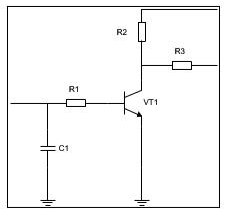
\includegraphics[width=0.3\linewidth]{image/schema1}
	\caption{Электрическая схема}
	\label{fig:schema1}
\end{figure}


\begin{table}[H]
	\caption{Перечень элементов}
	\label{tab:element_list}
	\begin{adjustbox}{width=\linewidth}
	\begin{tabular}{|c|c|c|c|c|}
		\hline
		№                  & Название схемы                           & \multicolumn{3}{c|}{Данные для расчета}                                     \\ \hline
		\multirow{6}{*}{1} & \multirow{6}{*}{Каскад входного фильтра} & Обозначение & Типономинал & Исходные данные                                 \\ \cline{3-5} 
		&                                          & R1          & Р1-16       & R=100 Ом, Р=3Вт, Рн=5 Вт, Допуск 10\%,Uмакс=5 В \\ \cline{3-5} 
		&                                          & R2          & C6-2        & R=200 Ом, Р=4Вт, Рн=6Вт, Допуск 5\%, Uмакс=6В   \\ \cline{3-5} 
		&                                          & R3          & Р2-75       & R=300 Ом, Р=3Вт, Рн=6Вт, Допуск 15\%,Uмакс=3 В  \\ \cline{3-5} 
		&                                          & C1          & К10-42      & С=10 мкФ, Uр=3В, Uном=5В                        \\ \cline{3-5} 
		&                                          & VT1         & 2Т203А      & Рр=4 Вт, Рмакс=6Вт, Нагрузка по напряжению 0,7  \\ \hline
	\end{tabular}
	\end{adjustbox}
\end{table}

\begin{table}[H]
	\caption{Показатели надежности электронных модулей}
	\label{tab:tab_2}
	\begin{adjustbox}{width=\linewidth}
	\begin{tabular}{|c|c|c|c|}
		\hline
		Наименование компонента & Дец. номер / Тип изделия & Эксплуатационная   интенсивность отказов & Интенсивность отказов в режиме ожидания \\ \hline
		VT1                     & 2T203A               & 2,01e-08                                 & 8,75e-11                                \\ \hline
		R1                      & Р1-16                     & 2,05e-07                                 & 4,82e-11                                \\ \hline
		R2                      & С6-2                     & 1,74e-08                                 & 3,64e-11                                \\ \hline
		R3                      & Р2-75                    & 1,35e-08                                 & 2,23e-10                                \\ \hline
		C1                      & К10-42                  & 3,38e-08                                 & 2,91e-10                                \\ \hline
	\end{tabular}
	\end{adjustbox}
\end{table}

\begin{figure}[H]
	\centering
	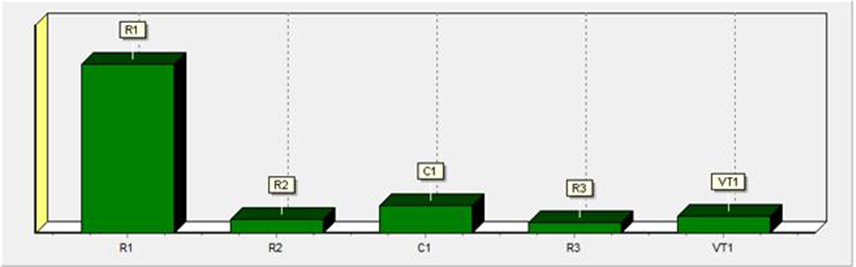
\includegraphics[width=0.7\linewidth]{image/graf}
	\caption{Вклады элементов в общую эксплуатационную интенсивность отказов}
	\label{fig:graf}
\end{figure}


\begin{figure}[H]
	\centering
	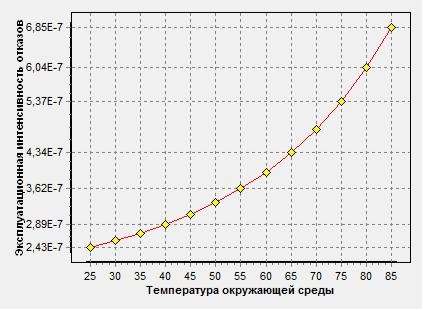
\includegraphics[width=0.6\linewidth]{image/temp}
	\caption{График зависимости эксплуатационной интенсивности отказов от температуры}
	\label{fig:temp}
\end{figure}



\section{Выводы по работе}

В ходе выполнения лабораторной работы были изучены математические модели интенсивности отказов ИЭТ, рассчитана надежность электронного модуля. 
Были построены графики зависимости эксплуатационной интенсивности отказов электронного модуля от температуры окружающей среды.

\section{Контрольные вопросы}

\begin{enumerate}

\item Какие сведения для расчета надежности приводятся для ИЭТ в справочниках по надежности?
\begin{itemize}
	\item номенклатуру ИЭТ, объединенных по общности их назначения,	основным параметрам и конструктивно-технологическому исполнению;
	\item условное обозначение ИЭТ;
	\item обозначение документа на поставку ИЭТ (ТУ, ОТУ);
	\item  математические модели (ММ) для расчета (прогнозирования)	значений эксплуатационной интенсивности отказов групп (типов) изделий, в том числе и при хранении в различных условиях;
	\item численные значения коэффициентов моделей.
\end{itemize}
 
\item Какая информация о показателях надежности ИЭТ и коэффициентах моделей приводиться в [6] на каждый класс?
\begin{itemize}
	\item значения интенсивности отказов групп (типов) ИЭТ при нормальной 	(максимально допустимой) температуре окружающей среды и номинальной электрической нагрузке или в типовых (усредненных) режимах
	эксплуатации;
	\item значения интенсивности отказов групп изделий при хранении в условиях отапливаемого хранилища в упаковке предприятия-изготовителя ИЭТ;
	\item количество отказов, по которым определены значения интенсивности отказов изделий;
	\item распределение отказов групп изделий по видам (по результатам проведения различных категорий испытаний);
	\item значения коэффициентов, входящих в модели прогнозирования эксплуатационной надежности ИЭТ, и аналитические выражения, показывающие зависимость этих коэффициентов от учитываемых факторов;
	\item нормируемые в технических условиях (экспериментально полученные) значения гамма-процентной наработки до отказа	(интенсивности отказов), гамма-процентного срока сохраняемости изделий;
	\item коэффициенты замен (среднестатистическую долю отказавших ИЭТ среди заменяемых в процессе поиска неисправности и ремонта аппаратуры) в условиях эксплуатации.
\end{itemize}
\item По каким математическим моделям рассчитывается эксплуатационная интенсивность отказов большинства ИЭТ из [8]?

Для проведения расчета надежности ИЭТ следует руководствоваться данными, приведенными в справочниках по надежности [3, 6-8]. 
Эти справочники имеют ряд отличий, как в структуре представления информации, так и в математических моделях интенсивностей отказов ИЭТ.

\item По какой математической модели рассчитывается эксплуатационная
интенсивность отказов отдельных групп сложных изделий в [7]?

Значения эксплуатационной интенсивности отказов (ИО) большинства
классов ИЭТ рассчитываются по математическим моделям, имеющим вид:

\begin{equation}
\lambda_{e} = \lambda_{b}^{'} K_p \prod_{i=1}^{n} K_i \text{~или~} \lambda_{e} = \lambda_{bcg}^{'} K_p \prod_{i=1}^{n} K_i
\end{equation}

\item Что характеризует коэффициент режима?

$K_p$ -- коэффициент режима, учитывающий изменение $\lambda_b^{'}(\lambda_{bcg}^{'})$ в зависимости от электрической нагрузки и (или)  $T_{okr}$; 

\item Что характеризует коэффициент приемки?

Коэффициент приемки ($K_{pr}$) отражает два уровня качества изготовления изделий: по справочнику [3], общее военное применение (ОВП) - приемка «5» и повышенной надежности (ОС) - приемка «9» (в эту же группу
входят изделия повышенной надежности, выпускаемые малыми партиями (ОСМ) -приемка «7»). Для изделий с приемкой «5» значение $K_{pr}$ принято равным 1.

\item Что характеризует коэффициент эксплуатации, и от чего он зависит?

Коэффициент эксплуатации ($K_{e}$) учитывает степень жесткости условий эксплуатации и показывает, во сколько раз интенсивность отказов ЭРИ в аппаратуре конкретного класса (группы эксплуатации по ГОСТ Р В 20.39.301-98) выше при всех прочих равных условиях, чем в наземной стационарной аппаратуре (группа 1.1). 
Для аппаратуры группы 1.1 значение коэффициента эксплуатации принято равным 1.

\item В чем суть разного подхода к построению отечественного и зарубежных справочников?

Зарубежные аналоги отечественного справочника имеют и другие кардинальные отличия. 
В частности, справочник, издаваемый МО США [6] имеет другую структуру. 
В нем нет типономиналов ИЭТ, а приведены лишь классы ИЭТ, группы, подгруппы и т.д.

\item Что такое идентификация?

Под идентификацией ИЭТ понимается классификация ИЭТ по справочникам, т.е. нахождение ММ исходя из конструктивных, технологических, электрических и др. параметров ИЭТ. 
Например, для идентификации микросхем необходимо знать технологическую группу (микросхемы памяти, микросхемы ПАВ и т.др.), количество выводов, объем бит, температуру перехода, рабочее напряжение, рассеиваемую мощность и т.д.
\end{enumerate}

\end{document} % конец документа


